\section{Regulator DMC}
\label{projekt:zad4}
-------POLECENIE--------

Napisac program w jezyku MATLAB do symulacji algorytm DMC w najprostszej
wersji analitycznej. Dobrac parametry D, Nu, N i lambda algorytmu DMC przy skokowej
zmianie sygnału wartosci zadanej z 0 do 1 i zerowym zakłóceniu. Jakosc regulacji
oceniac jakosciowo (na podstawie rysunków przebiegów sygnałów) oraz ilosciowo, wyznaczajac
wskaznik jakosci regulacji
E =
kXkonc
k=1
$(yzad(k) - y(k))2$
gdzie kkonc oznacza koniec symulacji (zawsze taki sam). Zamiescic wybrane wyniki
symulacji (przebiegi sygnałów wejsciowych i wyjsciowych procesu oraz wartosci wskaznika
E).

to samo co w proj 1

-------POLECENIE--------


Algorytm DMC (Dynamic Matrix Control) algorytm regulacji predykcyjnej. 
Do predykcji wykorzystuje się model procesu w postaci odpowiedzi skokowych. 
W algorytmie DMC dynamika obiektu regulacji modelowana jest dyskretnymi odpowiedziami skokowymi, 
które opisują reakcję wyjścia na skok jednostkowy sygnału sterującego.
 
% \begin{figure}[H]
%     \centering
%     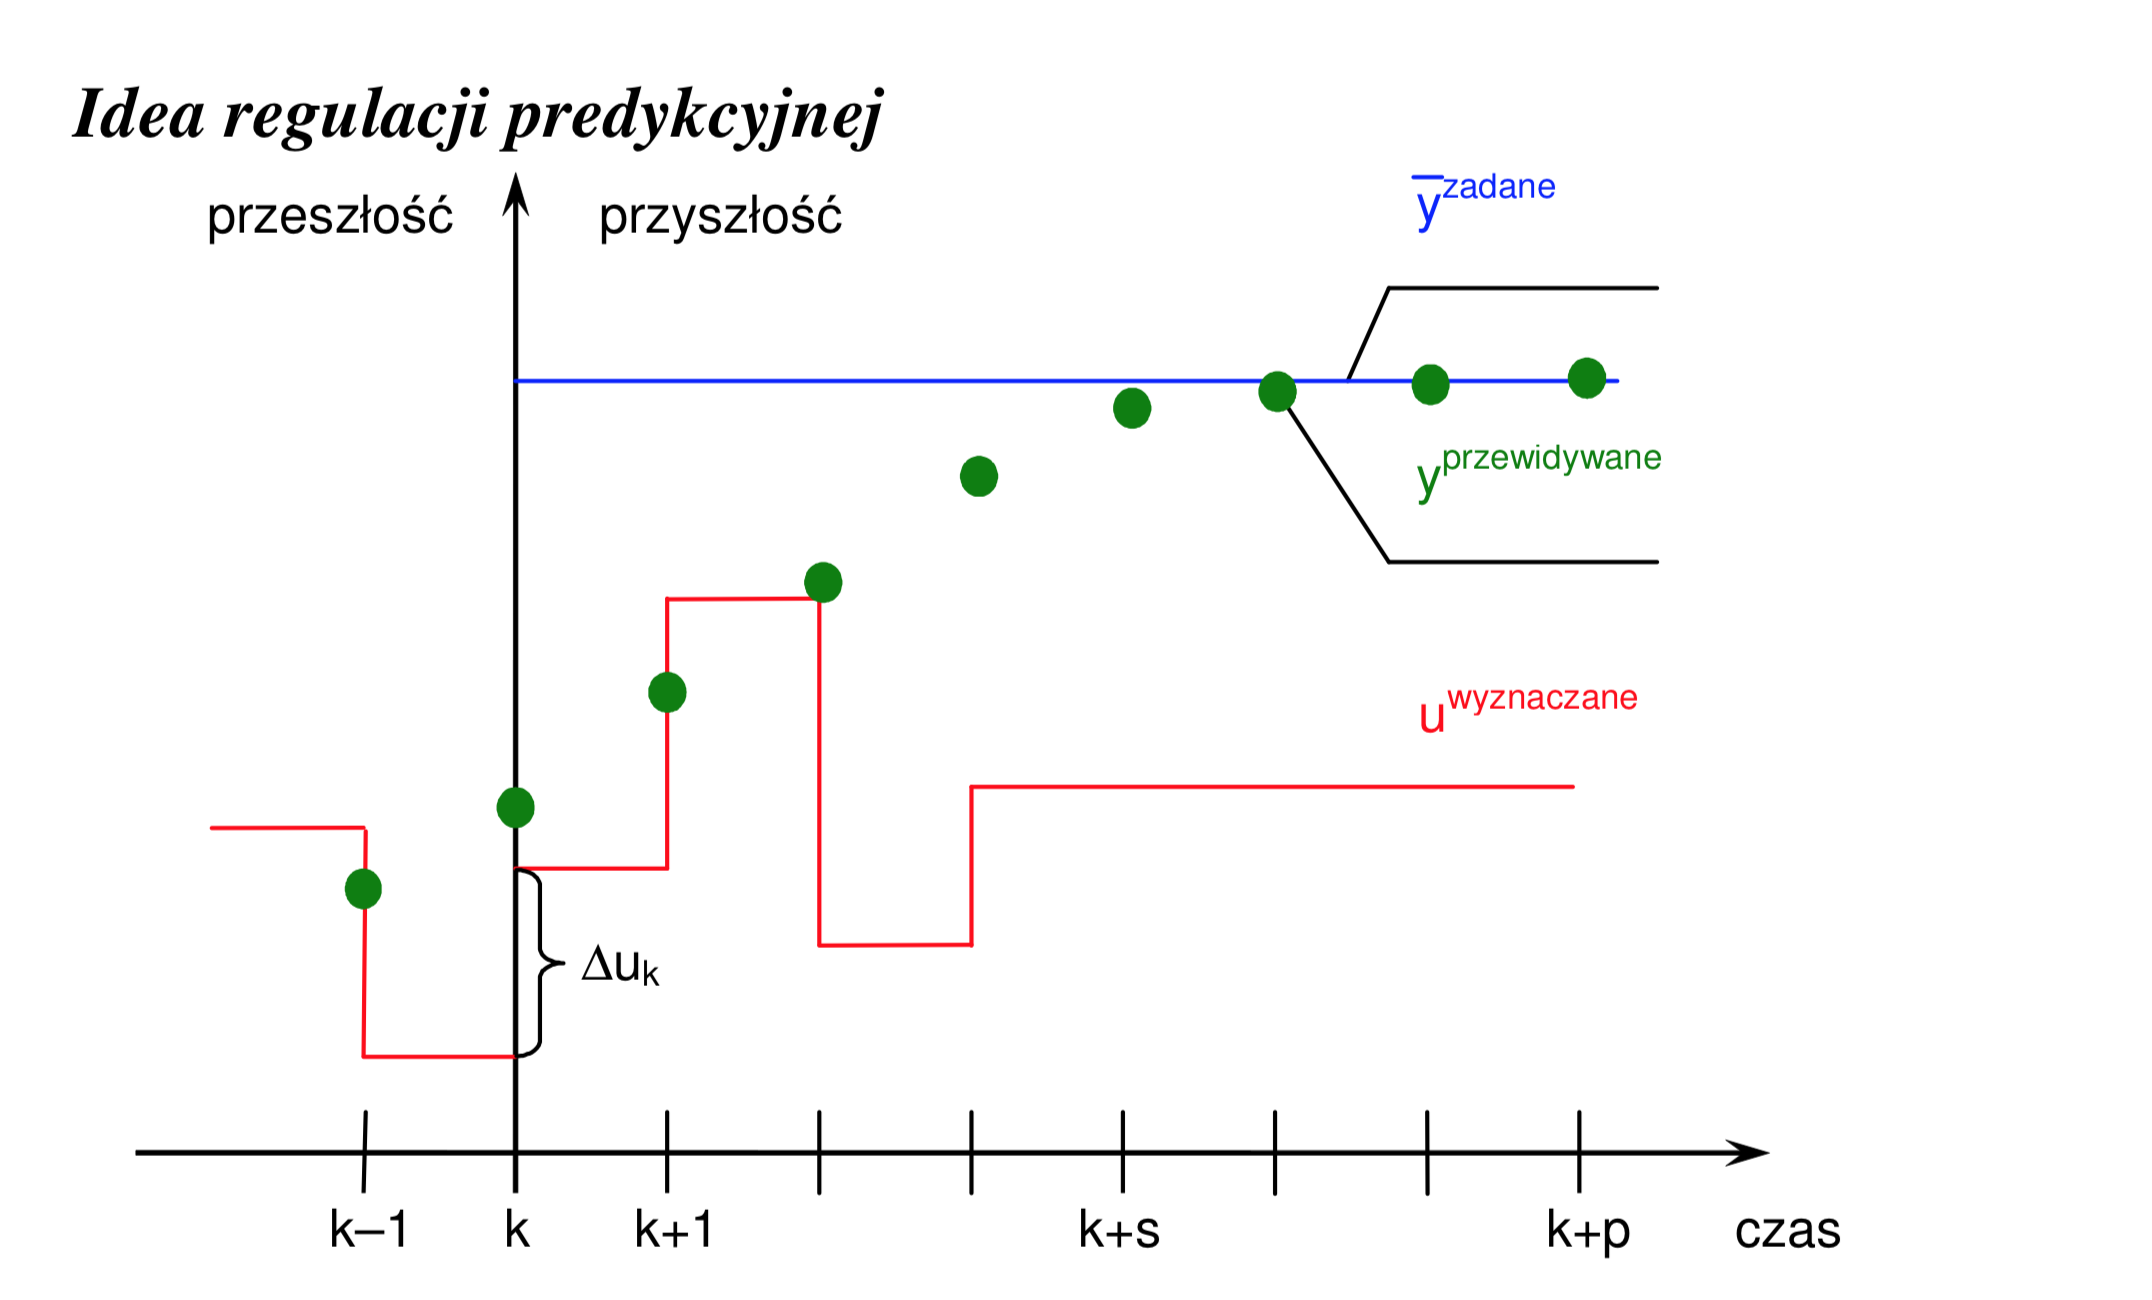
\includegraphics[scale=0.25]{dmc_idea.png}
%     \caption{Idea działania regulatora DMC}
% \end{figure}


\subsection{Program do symulacji algorytmu DMC}
\label{projekt:zad4:programDMC}

\subsection{Dobór parametrów regulatora}
\label{projekt:zad4:parametry}

\begin{figure}[H] 
    \centering
    % This file was created by matlab2tikz.
%
\definecolor{mycolor1}{rgb}{0.00000,0.44700,0.74100}%
\definecolor{mycolor2}{rgb}{0.85000,0.32500,0.09800}%
%
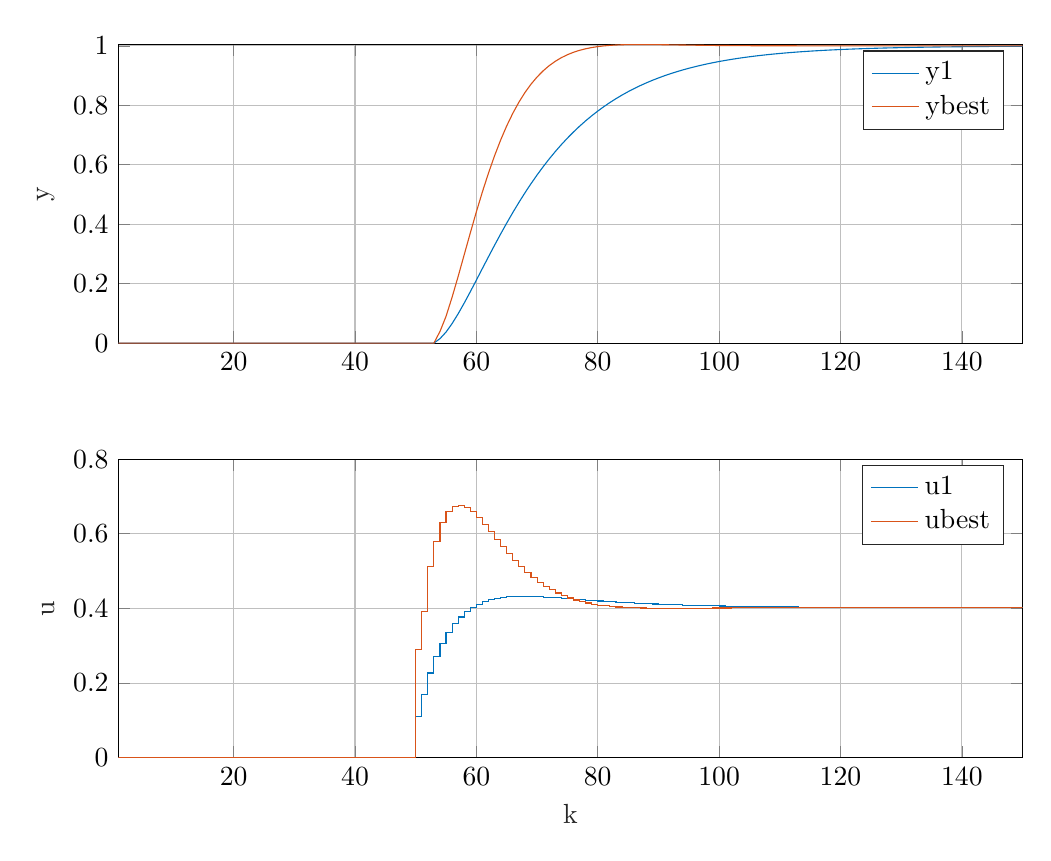
\begin{tikzpicture}

\begin{axis}[%
width=4.521in,
height=1.493in,
at={(0.758in,2.554in)},
scale only axis,
xmin=1,
xmax=150,
ymin=0,
ymax=1.0044,
ylabel style={font=\color{white!15!black}},
ylabel={y},
axis background/.style={fill=white},
xmajorgrids,
ymajorgrids,
legend style={legend cell align=left, align=left, draw=white!15!black}
]
\addplot [color=mycolor1]
  table[row sep=crcr]{%
1	0\\
2	0\\
3	0\\
4	0\\
5	0\\
6	0\\
7	0\\
8	0\\
9	0\\
10	0\\
11	0\\
12	0\\
13	0\\
14	0\\
15	0\\
16	0\\
17	0\\
18	0\\
19	0\\
20	0\\
21	0\\
22	0\\
23	0\\
24	0\\
25	0\\
26	0\\
27	0\\
28	0\\
29	0\\
30	0\\
31	0\\
32	0\\
33	0\\
34	0\\
35	0\\
36	0\\
37	0\\
38	0\\
39	0\\
40	0\\
41	0\\
42	0\\
43	0\\
44	0\\
45	0\\
46	0\\
47	0\\
48	0\\
49	0\\
50	0\\
51	0\\
52	0\\
53	0\\
54	0.014971\\
55	0.037108\\
56	0.065743\\
57	0.098732\\
58	0.13481\\
59	0.17282\\
60	0.2119\\
61	0.25135\\
62	0.29063\\
63	0.32931\\
64	0.36708\\
65	0.40371\\
66	0.43903\\
67	0.47292\\
68	0.50531\\
69	0.53615\\
70	0.56545\\
71	0.5932\\
72	0.61943\\
73	0.64419\\
74	0.6675\\
75	0.68944\\
76	0.71004\\
77	0.72938\\
78	0.74751\\
79	0.76449\\
80	0.78039\\
81	0.79527\\
82	0.80917\\
83	0.82216\\
84	0.8343\\
85	0.84563\\
86	0.8562\\
87	0.86607\\
88	0.87527\\
89	0.88385\\
90	0.89185\\
91	0.89931\\
92	0.90626\\
93	0.91273\\
94	0.91876\\
95	0.92438\\
96	0.92961\\
97	0.93449\\
98	0.93903\\
99	0.94325\\
100	0.94719\\
101	0.95085\\
102	0.95426\\
103	0.95743\\
104	0.96039\\
105	0.96314\\
106	0.9657\\
107	0.96808\\
108	0.9703\\
109	0.97236\\
110	0.97428\\
111	0.97607\\
112	0.97773\\
113	0.97928\\
114	0.98072\\
115	0.98206\\
116	0.98331\\
117	0.98447\\
118	0.98555\\
119	0.98655\\
120	0.98749\\
121	0.98836\\
122	0.98917\\
123	0.98992\\
124	0.99062\\
125	0.99127\\
126	0.99188\\
127	0.99245\\
128	0.99297\\
129	0.99346\\
130	0.99392\\
131	0.99434\\
132	0.99473\\
133	0.9951\\
134	0.99544\\
135	0.99576\\
136	0.99605\\
137	0.99633\\
138	0.99658\\
139	0.99682\\
140	0.99704\\
141	0.99725\\
142	0.99744\\
143	0.99762\\
144	0.99778\\
145	0.99794\\
146	0.99808\\
147	0.99821\\
148	0.99834\\
149	0.99845\\
150	0.99856\\
151	0.99866\\
152	0.99876\\
153	0.99884\\
154	0.99892\\
155	0.999\\
156	0.99907\\
157	0.99913\\
158	0.99919\\
159	0.99925\\
160	0.9993\\
161	0.99935\\
162	0.9994\\
163	0.99944\\
164	0.99948\\
165	0.99952\\
166	0.99955\\
167	0.99958\\
168	0.99961\\
169	0.99964\\
170	0.99966\\
171	0.99969\\
172	0.99971\\
173	0.99973\\
174	0.99975\\
175	0.99977\\
176	0.99979\\
177	0.9998\\
178	0.99982\\
179	0.99983\\
180	0.99984\\
181	0.99986\\
182	0.99987\\
183	0.99988\\
184	0.99989\\
185	0.9999\\
186	0.9999\\
187	0.99991\\
188	0.99992\\
189	0.99993\\
190	0.99993\\
191	0.99994\\
192	0.99994\\
193	0.99995\\
194	0.99996\\
195	0.99996\\
196	0.99996\\
197	0.99997\\
198	0.99997\\
199	0.99998\\
200	0.99998\\
201	0.99998\\
202	0.99999\\
203	0.99999\\
204	0.99999\\
205	0.99999\\
206	1\\
207	1\\
208	1\\
209	1\\
210	1\\
211	1\\
212	1\\
213	1\\
214	1\\
215	1\\
216	1\\
217	1\\
218	1\\
219	1\\
220	1\\
221	1\\
222	1\\
223	1\\
224	1\\
225	1\\
226	1\\
227	1\\
228	1\\
229	1\\
230	1\\
231	1\\
232	1\\
233	1\\
234	1\\
235	1\\
236	1\\
237	1\\
238	1\\
239	1\\
240	1\\
241	1\\
242	1\\
243	1\\
244	1\\
245	1\\
246	1\\
247	1\\
248	1\\
249	1\\
250	1\\
251	1\\
252	1\\
253	1\\
254	1\\
255	1\\
256	1\\
257	1\\
258	1\\
259	1\\
260	1\\
261	1\\
262	1\\
263	1\\
264	1\\
265	1\\
266	1\\
267	1\\
268	1\\
269	1\\
270	1\\
271	1\\
272	1\\
273	1\\
274	1\\
275	1\\
276	1\\
277	1\\
278	1\\
279	1\\
280	1\\
281	1\\
282	1\\
283	1\\
284	1\\
285	1\\
286	1\\
287	1\\
288	1\\
289	1\\
290	1\\
291	1\\
292	1\\
293	1\\
294	1\\
295	1\\
296	1\\
297	1\\
298	1\\
299	1\\
300	1\\
};
\addlegendentry{y1}

\addplot [color=mycolor2]
  table[row sep=crcr]{%
1	0\\
2	0\\
3	0\\
4	0\\
5	0\\
6	0\\
7	0\\
8	0\\
9	0\\
10	0\\
11	0\\
12	0\\
13	0\\
14	0\\
15	0\\
16	0\\
17	0\\
18	0\\
19	0\\
20	0\\
21	0\\
22	0\\
23	0\\
24	0\\
25	0\\
26	0\\
27	0\\
28	0\\
29	0\\
30	0\\
31	0\\
32	0\\
33	0\\
34	0\\
35	0\\
36	0\\
37	0\\
38	0\\
39	0\\
40	0\\
41	0\\
42	0\\
43	0\\
44	0\\
45	0\\
46	0\\
47	0\\
48	0\\
49	0\\
50	0\\
51	0\\
52	0\\
53	0\\
54	0.039119\\
55	0.090032\\
56	0.15448\\
57	0.22449\\
58	0.29764\\
59	0.37063\\
60	0.44164\\
61	0.50914\\
62	0.57223\\
63	0.63032\\
64	0.68313\\
65	0.73061\\
66	0.77286\\
67	0.81011\\
68	0.84266\\
69	0.87086\\
70	0.8951\\
71	0.91576\\
72	0.93322\\
73	0.94786\\
74	0.96003\\
75	0.97004\\
76	0.97821\\
77	0.98479\\
78	0.99003\\
79	0.99414\\
80	0.99731\\
81	0.99971\\
82	1.0015\\
83	1.0027\\
84	1.0036\\
85	1.0041\\
86	1.0043\\
87	1.0044\\
88	1.0043\\
89	1.0042\\
90	1.0039\\
91	1.0036\\
92	1.0033\\
93	1.003\\
94	1.0027\\
95	1.0024\\
96	1.0021\\
97	1.0018\\
98	1.0016\\
99	1.0013\\
100	1.0011\\
101	1.001\\
102	1.0008\\
103	1.0007\\
104	1.0005\\
105	1.0004\\
106	1.0003\\
107	1.0003\\
108	1.0002\\
109	1.0002\\
110	1.0001\\
111	1.0001\\
112	1.0001\\
113	1\\
114	1\\
115	1\\
116	1\\
117	0.99999\\
118	0.99998\\
119	0.99998\\
120	0.99998\\
121	0.99998\\
122	0.99998\\
123	0.99998\\
124	0.99998\\
125	0.99998\\
126	0.99998\\
127	0.99998\\
128	0.99998\\
129	0.99998\\
130	0.99998\\
131	0.99998\\
132	0.99999\\
133	0.99999\\
134	0.99999\\
135	0.99999\\
136	0.99999\\
137	0.99999\\
138	0.99999\\
139	0.99999\\
140	0.99999\\
141	0.99999\\
142	0.99999\\
143	0.99999\\
144	0.99999\\
145	0.99999\\
146	0.99999\\
147	0.99999\\
148	0.99999\\
149	0.99999\\
150	0.99999\\
151	0.99999\\
152	0.99999\\
153	0.99999\\
154	0.99999\\
155	0.99999\\
156	0.99999\\
157	0.99999\\
158	0.99999\\
159	0.99999\\
160	0.99999\\
161	0.99999\\
162	0.99999\\
163	0.99999\\
164	0.99999\\
165	0.99999\\
166	0.99999\\
167	0.99999\\
168	0.99999\\
169	0.99999\\
170	0.99999\\
171	0.99999\\
172	0.99999\\
173	0.99999\\
174	0.99999\\
175	0.99999\\
176	0.99999\\
177	0.99999\\
178	0.99999\\
179	0.99999\\
180	0.99999\\
181	0.99999\\
182	0.99999\\
183	0.99999\\
184	0.99999\\
185	0.99999\\
186	0.99999\\
187	0.99999\\
188	0.99999\\
189	0.99999\\
190	0.99999\\
191	0.99999\\
192	0.99999\\
193	0.99999\\
194	0.99999\\
195	0.99999\\
196	0.99999\\
197	0.99999\\
198	0.99999\\
199	0.99999\\
200	0.99999\\
201	0.99999\\
202	0.99999\\
203	0.99999\\
204	0.99999\\
205	0.99999\\
206	0.99999\\
207	0.99999\\
208	1\\
209	1\\
210	1\\
211	1\\
212	1\\
213	1\\
214	1\\
215	1\\
216	1\\
217	1\\
218	1\\
219	1\\
220	1\\
221	1\\
222	1\\
223	1\\
224	1\\
225	1\\
226	1\\
227	1\\
228	1\\
229	1\\
230	1\\
231	1\\
232	1\\
233	1\\
234	1\\
235	1\\
236	1\\
237	1\\
238	1\\
239	1\\
240	1\\
241	1\\
242	1\\
243	1\\
244	1\\
245	1\\
246	1\\
247	1\\
248	1\\
249	1\\
250	1\\
251	1\\
252	1\\
253	1\\
254	1\\
255	1\\
256	1\\
257	1\\
258	1\\
259	1\\
260	1\\
261	1\\
262	1\\
263	1\\
264	1\\
265	1\\
266	1\\
267	1\\
268	1\\
269	1\\
270	1\\
271	1\\
272	1\\
273	1\\
274	1\\
275	1\\
276	1\\
277	1\\
278	1\\
279	1\\
280	1\\
281	1\\
282	1\\
283	1\\
284	1\\
285	1\\
286	1\\
287	1\\
288	1\\
289	1\\
290	1\\
291	1\\
292	1\\
293	1\\
294	1\\
295	1\\
296	1\\
297	1\\
298	1\\
299	1\\
300	1\\
};
\addlegendentry{ybest}

\end{axis}

\begin{axis}[%
width=4.521in,
height=1.493in,
at={(0.758in,0.481in)},
scale only axis,
xmin=1,
xmax=150,
xlabel style={font=\color{white!15!black}},
xlabel={k},
ymin=0,
ymax=0.8,
ylabel style={font=\color{white!15!black}},
ylabel={u},
axis background/.style={fill=white},
xmajorgrids,
ymajorgrids,
legend style={legend cell align=left, align=left, draw=white!15!black}
]
\addplot[const plot, color=mycolor1] table[row sep=crcr] {%
1	0\\
2	0\\
3	0\\
4	0\\
5	0\\
6	0\\
7	0\\
8	0\\
9	0\\
10	0\\
11	0\\
12	0\\
13	0\\
14	0\\
15	0\\
16	0\\
17	0\\
18	0\\
19	0\\
20	0\\
21	0\\
22	0\\
23	0\\
24	0\\
25	0\\
26	0\\
27	0\\
28	0\\
29	0\\
30	0\\
31	0\\
32	0\\
33	0\\
34	0\\
35	0\\
36	0\\
37	0\\
38	0\\
39	0\\
40	0\\
41	0\\
42	0\\
43	0\\
44	0\\
45	0\\
46	0\\
47	0\\
48	0\\
49	0\\
50	0.11082\\
51	0.16985\\
52	0.22681\\
53	0.27051\\
54	0.30656\\
55	0.33537\\
56	0.35851\\
57	0.37691\\
58	0.39144\\
59	0.40281\\
60	0.41159\\
61	0.41828\\
62	0.42326\\
63	0.42686\\
64	0.42935\\
65	0.43096\\
66	0.43187\\
67	0.43221\\
68	0.43212\\
69	0.4317\\
70	0.43102\\
71	0.43015\\
72	0.42915\\
73	0.42805\\
74	0.42689\\
75	0.4257\\
76	0.4245\\
77	0.4233\\
78	0.42212\\
79	0.42097\\
80	0.41986\\
81	0.41878\\
82	0.41775\\
83	0.41676\\
84	0.41582\\
85	0.41493\\
86	0.41409\\
87	0.41329\\
88	0.41253\\
89	0.41182\\
90	0.41116\\
91	0.41053\\
92	0.40994\\
93	0.40939\\
94	0.40887\\
95	0.40839\\
96	0.40794\\
97	0.40751\\
98	0.40712\\
99	0.40675\\
100	0.4064\\
101	0.40608\\
102	0.40578\\
103	0.4055\\
104	0.40524\\
105	0.405\\
106	0.40477\\
107	0.40456\\
108	0.40436\\
109	0.40418\\
110	0.40401\\
111	0.40385\\
112	0.4037\\
113	0.40357\\
114	0.40344\\
115	0.40332\\
116	0.40321\\
117	0.4031\\
118	0.40301\\
119	0.40292\\
120	0.40283\\
121	0.40276\\
122	0.40268\\
123	0.40262\\
124	0.40255\\
125	0.4025\\
126	0.40244\\
127	0.40239\\
128	0.40234\\
129	0.4023\\
130	0.40226\\
131	0.40222\\
132	0.40219\\
133	0.40215\\
134	0.40212\\
135	0.40209\\
136	0.40207\\
137	0.40204\\
138	0.40202\\
139	0.402\\
140	0.40198\\
141	0.40196\\
142	0.40194\\
143	0.40193\\
144	0.40191\\
145	0.4019\\
146	0.40189\\
147	0.40188\\
148	0.40186\\
149	0.40185\\
150	0.40185\\
151	0.40184\\
152	0.40183\\
153	0.40182\\
154	0.40181\\
155	0.40181\\
156	0.4018\\
157	0.4018\\
158	0.40179\\
159	0.40179\\
160	0.40178\\
161	0.40178\\
162	0.40177\\
163	0.40177\\
164	0.40177\\
165	0.40176\\
166	0.40176\\
167	0.40176\\
168	0.40175\\
169	0.40175\\
170	0.40175\\
171	0.40175\\
172	0.40175\\
173	0.40175\\
174	0.40174\\
175	0.40174\\
176	0.40174\\
177	0.40174\\
178	0.40174\\
179	0.40174\\
180	0.40174\\
181	0.40174\\
182	0.40174\\
183	0.40173\\
184	0.40173\\
185	0.40173\\
186	0.40173\\
187	0.40173\\
188	0.40173\\
189	0.40173\\
190	0.40173\\
191	0.40173\\
192	0.40173\\
193	0.40173\\
194	0.40173\\
195	0.40173\\
196	0.40173\\
197	0.40173\\
198	0.40173\\
199	0.40173\\
200	0.40173\\
201	0.40173\\
202	0.40173\\
203	0.40173\\
204	0.40173\\
205	0.40173\\
206	0.40173\\
207	0.40173\\
208	0.40173\\
209	0.40173\\
210	0.40173\\
211	0.40173\\
212	0.40173\\
213	0.40173\\
214	0.40173\\
215	0.40173\\
216	0.40173\\
217	0.40173\\
218	0.40173\\
219	0.40173\\
220	0.40173\\
221	0.40173\\
222	0.40173\\
223	0.40173\\
224	0.40173\\
225	0.40173\\
226	0.40173\\
227	0.40173\\
228	0.40173\\
229	0.40173\\
230	0.40173\\
231	0.40173\\
232	0.40173\\
233	0.40173\\
234	0.40173\\
235	0.40173\\
236	0.40173\\
237	0.40173\\
238	0.40173\\
239	0.40173\\
240	0.40173\\
241	0.40173\\
242	0.40173\\
243	0.40173\\
244	0.40173\\
245	0.40173\\
246	0.40173\\
247	0.40172\\
248	0.40172\\
249	0.40172\\
250	0.40172\\
251	0.40172\\
252	0.40172\\
253	0.40172\\
254	0.40172\\
255	0.40172\\
256	0.40172\\
257	0.40172\\
258	0.40172\\
259	0.40172\\
260	0.40172\\
261	0.40172\\
262	0.40172\\
263	0.40172\\
264	0.40172\\
265	0.40172\\
266	0.40172\\
267	0.40172\\
268	0.40172\\
269	0.40172\\
270	0.40172\\
271	0.40172\\
272	0.40172\\
273	0.40172\\
274	0.40172\\
275	0.40172\\
276	0.40172\\
277	0.40172\\
278	0.40172\\
279	0.40172\\
280	0.40172\\
281	0.40172\\
282	0.40172\\
283	0.40172\\
284	0.40172\\
285	0.40172\\
286	0.40172\\
287	0.40172\\
288	0.40172\\
289	0.40172\\
290	0.40172\\
291	0.40172\\
292	0.40172\\
293	0.40172\\
294	0.40172\\
295	0.40172\\
296	0.40172\\
297	0.40172\\
298	0.40172\\
299	0.40172\\
300	0.40172\\
};
\addlegendentry{u1}

\addplot[const plot, color=mycolor2] table[row sep=crcr] {%
1	0\\
2	0\\
3	0\\
4	0\\
5	0\\
6	0\\
7	0\\
8	0\\
9	0\\
10	0\\
11	0\\
12	0\\
13	0\\
14	0\\
15	0\\
16	0\\
17	0\\
18	0\\
19	0\\
20	0\\
21	0\\
22	0\\
23	0\\
24	0\\
25	0\\
26	0\\
27	0\\
28	0\\
29	0\\
30	0\\
31	0\\
32	0\\
33	0\\
34	0\\
35	0\\
36	0\\
37	0\\
38	0\\
39	0\\
40	0\\
41	0\\
42	0\\
43	0\\
44	0\\
45	0\\
46	0\\
47	0\\
48	0\\
49	0\\
50	0.28956\\
51	0.39251\\
52	0.5131\\
53	0.58007\\
54	0.63135\\
55	0.65951\\
56	0.67407\\
57	0.67664\\
58	0.67103\\
59	0.65931\\
60	0.64358\\
61	0.62529\\
62	0.60567\\
63	0.58562\\
64	0.56581\\
65	0.54674\\
66	0.52873\\
67	0.512\\
68	0.49669\\
69	0.48283\\
70	0.47042\\
71	0.45942\\
72	0.44977\\
73	0.44136\\
74	0.4341\\
75	0.42788\\
76	0.4226\\
77	0.41815\\
78	0.41444\\
79	0.41136\\
80	0.40884\\
81	0.4068\\
82	0.40516\\
83	0.40387\\
84	0.40286\\
85	0.40209\\
86	0.40151\\
87	0.4011\\
88	0.40081\\
89	0.40063\\
90	0.40052\\
91	0.40048\\
92	0.40048\\
93	0.40051\\
94	0.40057\\
95	0.40065\\
96	0.40073\\
97	0.40082\\
98	0.40091\\
99	0.401\\
100	0.40108\\
101	0.40116\\
102	0.40123\\
103	0.4013\\
104	0.40136\\
105	0.40142\\
106	0.40146\\
107	0.4015\\
108	0.40154\\
109	0.40157\\
110	0.4016\\
111	0.40162\\
112	0.40164\\
113	0.40166\\
114	0.40167\\
115	0.40168\\
116	0.40169\\
117	0.4017\\
118	0.4017\\
119	0.40171\\
120	0.40171\\
121	0.40171\\
122	0.40171\\
123	0.40172\\
124	0.40172\\
125	0.40172\\
126	0.40172\\
127	0.40172\\
128	0.40172\\
129	0.40172\\
130	0.40172\\
131	0.40172\\
132	0.40172\\
133	0.40171\\
134	0.40171\\
135	0.40171\\
136	0.40171\\
137	0.40171\\
138	0.40171\\
139	0.40171\\
140	0.40171\\
141	0.40171\\
142	0.40171\\
143	0.40171\\
144	0.40171\\
145	0.40171\\
146	0.40171\\
147	0.40171\\
148	0.40171\\
149	0.40171\\
150	0.40171\\
151	0.40171\\
152	0.40171\\
153	0.40171\\
154	0.40171\\
155	0.40171\\
156	0.40171\\
157	0.40171\\
158	0.40171\\
159	0.40171\\
160	0.40171\\
161	0.40171\\
162	0.40171\\
163	0.40171\\
164	0.40171\\
165	0.40171\\
166	0.40171\\
167	0.40171\\
168	0.40171\\
169	0.40171\\
170	0.40171\\
171	0.40171\\
172	0.40171\\
173	0.40171\\
174	0.40171\\
175	0.40171\\
176	0.40171\\
177	0.40171\\
178	0.40171\\
179	0.40171\\
180	0.40171\\
181	0.40171\\
182	0.40171\\
183	0.40171\\
184	0.40171\\
185	0.40171\\
186	0.40171\\
187	0.40171\\
188	0.40171\\
189	0.40171\\
190	0.40171\\
191	0.40171\\
192	0.40171\\
193	0.40171\\
194	0.40171\\
195	0.40171\\
196	0.40171\\
197	0.40171\\
198	0.40171\\
199	0.40171\\
200	0.40171\\
201	0.40172\\
202	0.40172\\
203	0.40172\\
204	0.40172\\
205	0.40172\\
206	0.40172\\
207	0.40172\\
208	0.40172\\
209	0.40172\\
210	0.40172\\
211	0.40172\\
212	0.40172\\
213	0.40172\\
214	0.40172\\
215	0.40172\\
216	0.40172\\
217	0.40172\\
218	0.40172\\
219	0.40173\\
220	0.40173\\
221	0.40173\\
222	0.40173\\
223	0.40173\\
224	0.40173\\
225	0.40173\\
226	0.40173\\
227	0.40174\\
228	0.40174\\
229	0.40174\\
230	0.40174\\
231	0.40174\\
232	0.40174\\
233	0.40174\\
234	0.40173\\
235	0.40173\\
236	0.40173\\
237	0.40173\\
238	0.40172\\
239	0.40172\\
240	0.40172\\
241	0.40172\\
242	0.40172\\
243	0.40172\\
244	0.40171\\
245	0.40171\\
246	0.40171\\
247	0.40171\\
248	0.40171\\
249	0.40171\\
250	0.40171\\
251	0.40171\\
252	0.40171\\
253	0.40171\\
254	0.40171\\
255	0.40171\\
256	0.40171\\
257	0.40171\\
258	0.40171\\
259	0.40171\\
260	0.40171\\
261	0.40171\\
262	0.40171\\
263	0.40171\\
264	0.40171\\
265	0.40171\\
266	0.40171\\
267	0.40171\\
268	0.40171\\
269	0.40171\\
270	0.40171\\
271	0.40171\\
272	0.40171\\
273	0.40171\\
274	0.40171\\
275	0.40171\\
276	0.40171\\
277	0.40171\\
278	0.40171\\
279	0.40171\\
280	0.40172\\
281	0.40172\\
282	0.40172\\
283	0.40172\\
284	0.40172\\
285	0.40172\\
286	0.40172\\
287	0.40172\\
288	0.40172\\
289	0.40172\\
290	0.40172\\
291	0.40172\\
292	0.40172\\
293	0.40172\\
294	0.40172\\
295	0.40172\\
296	0.40172\\
297	0.40172\\
298	0.40172\\
299	0.40172\\
300	0.40172\\
};
\addlegendentry{ubest}

\end{axis}
\end{tikzpicture}%
    \caption{Przebiegi dla różnych nastaw regulatorów}
    \label{projekt:zad4:parametry:figure}
\end{figure}
